\documentclass[11pt]{article}
\usepackage{acl2014}
\usepackage{times}
\usepackage{url}
\usepackage{latexsym}

\usepackage{graphicx}
\usepackage{hyperref}
\usepackage{bera}% optional: just to have a nice mono-spaced font
\usepackage{listings}
\usepackage{xcolor}

\colorlet{punct}{red!60!black}
\definecolor{background}{HTML}{EEEEEE}
\definecolor{delim}{RGB}{20,105,176}
\colorlet{numb}{magenta!60!black}

\lstdefinelanguage{json}{
	basicstyle=\normalfont\ttfamily,
	numbers=left,
	numberstyle=\scriptsize,
	stepnumber=1,
	numbersep=8pt,
	showstringspaces=false,
	breaklines=true,
	frame=lines,
	backgroundcolor=\color{background},
	literate=
	*{0}{{{\color{numb}0}}}{1}
	{1}{{{\color{numb}1}}}{1}
	{2}{{{\color{numb}2}}}{1}
	{3}{{{\color{numb}3}}}{1}
	{4}{{{\color{numb}4}}}{1}
	{5}{{{\color{numb}5}}}{1}
	{6}{{{\color{numb}6}}}{1}
	{7}{{{\color{numb}7}}}{1}
	{8}{{{\color{numb}8}}}{1}
	{9}{{{\color{numb}9}}}{1}
	{:}{{{\color{punct}{:}}}}{1}
	{,}{{{\color{punct}{,}}}}{1}
	{\{}{{{\color{delim}{\{}}}}{1}
	{\}}{{{\color{delim}{\}}}}}{1}
	{[}{{{\color{delim}{[}}}}{1}
	{]}{{{\color{delim}{]}}}}{1},
}

\setlength\titlebox{5cm}

% You can expand the titlebox if you need extra space
% to show all the authors. Please do not make the titlebox
% smaller than 5cm (the original size); we will check this
% in the camera-ready version and ask you to change it back.


\title{Project Echo}

\author{
Dídac Fernández Cadenas\\
{\tt didac.fernandezcadenas@epfl.ch} \\
\textbf{Vikalp Kamdar}\\
{\tt vikalp.kamdar@epfl.ch} \\
\textbf{Jorge Sánchez González}\\
{\tt jorge.sanchezgonzalez@epfl.ch} \\}

\date{}

\begin{document}
\maketitle
\begin{abstract}
 In this project we mine data from a public database of Reddit comments and use it to observe and understand better the echo chamber effect. We perform an observational study on the interaction between Reddit communities centered around political discussion. More precisely, we are interested in social engineering and leveraging the effect to guess the ideology of users based on this public data. We introduce several different approaches to that problem.
\end{abstract}

\section{Introduction}

\subsection{The Echo Chamber Effect}

We call a community an echo chamber when a group that shows built-in biases, traits, opinions, etc. (so any group) interacts relatively only within itself, self-reinforcing those opinions and biases.

Echo chambers are constituted by a mix of homophily (similar individuals are brought together) and influence (they influence each other, reinforcing those traits they share). 

The ease of access of the internet makes homophily effortless, a user only needs to perform a single Google query to find a community of like-minded individuals. Furthermore, it is easy to filter out content we don't agree with or that we just don't want to see. This creates a self-sorting effect in online communities.

The structured nature of mass social media makes influence powerful and exploitable. It is much easier for some individuals (the influencers, high degree nodes of the network) to spread their opinions, and communities will form around them and their ideologies. Likewise, it is (many orders of magnitude) easier than ever to gather mass data about social interaction to monitor or artificially influence those communities.

\subsection{Reddit}

There are two main components to the Reddit structure: the communities or \textbf{subreddits} and the \textbf{voting system} (or karma system).

There is no recommender system. People vote on what is relevant so if a majority are wrong, biased, or someone with the means gets enough people to believe something, then that something becomes the relevant discussion topic. The karma system is both the greatest advantage and the single point of failure of Reddit.

\subsection{The Dataset}

Our dataset of choice consists on all the comments in Reddit from its inception in 2005 to March 2017.

The dataset is a list of JSON objects with comments, as well as several identifiers and information about them.

It should be noted that over the years the structure has changed slightly and some fields are not present throughout the whole dataset but since we restrict ourselves to a small time period and only some fields that was not a problem in our case.
A detailed explanation of each field can be found in the github's README.

\subsection{Sifting Through the Data}

To focus in a single example we take a look at Reddit during the US presidential election in 2016, knowing that the event prompted a lot social engineering attempts from the candidates' campaign teams and possibly other external agents. 

We used the IC Cluster and Apache Spark to perform some filters, outlier removal (like exceedingly large subreddits or very irrelevant comments, like numbers), and cleaning (removal of [deleted] usernames and comments or JSON fields that don't help us).

After that, we randomly sampled 1 million users and retrieved all of their comments as the main dataset. This means around 64 million comments total.

From those (and in order to be able to work locally with the usual tools) we focus in politics: we take only comments by users who have commented at least once in one of the 8 subreddits about politics, bringing it down to around 28 million comments.

As additional datapoints we extracted small samples from certain subreddits dedicated to political ideologies (see \href{https://www.reddit.com/r/redditlists/comments/josdr/list_of_political_subreddits/}{this list} from r/redditlists)	

\section{Scanning for Echo Chambers}

The first part of the project consists in observing the behaviour of the network and how communities interact. We will look at our politics-themed subreddits and their interactions.

\subsection{Visualizing the Network}
We take subreddits as nodes and build a weighted adjacency matrix with the number of users that cross-post between two subreddits as the weight. In this state it is still hard to interpret anything since the edges are bidirectional and the weights are heavily biased by the size of each node, as we can see in fig. \ref{base_net} (Fig. \ref{base_net_big} in the appendix for bigger size).

\begin{figure}[h]
	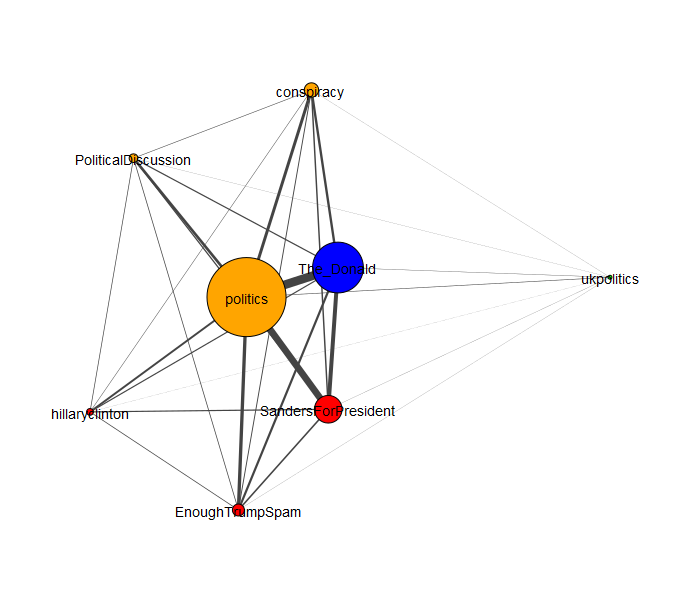
\includegraphics[width=\columnwidth]{img/base_network.png}
	\caption{\label{base_net} Base network model}
\end{figure}
 
\subsection{Fine-tuning the Network}
To look at how subreddit A interacts with subreddit B we would like a one-sided measure of interaction. With this in mind we assign a "main" subreddit to each user, add up all karma that each user has in each subreddit, and the one with the highest score will be it's home sub. This represents the fact that this community aligns with the user and viceversa.

The second problem with fig. \ref{base_net} is that edge size is heavily correlated with the size of the nodes, polluting our precious insight. To correct for that, we instead look at the percentage of sub A users that commented on sub B. The result, in fig. \ref{karma_net} (Fig. \ref{karma_net_big} in the appendix).

\begin{figure}[h]
	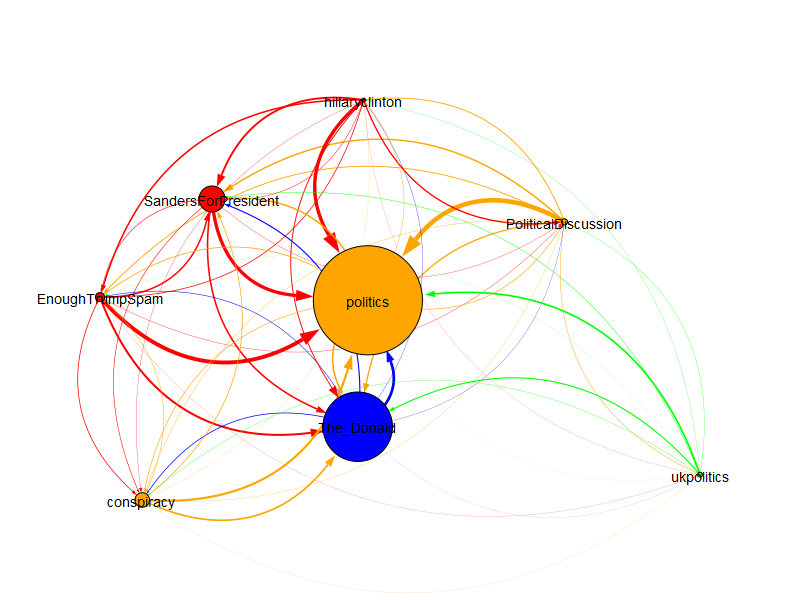
\includegraphics[width=\columnwidth]{img/karma_model.png}
	\caption{\label{karma_net} Karma model in political subs}
\end{figure}

\subsection{Political Ideologies in Isolation}

In figure \ref{ideology_net} (Fig. \ref{ideology_net_big} in the appendix) we can see our model applied to some of the ideology-centric communities on Reddit. On average, only $2\%$ of each community went on and commented in a particular other. We can appreciate that similar ideologies have stronger ties. The most interesting though is that, in general, the right is clustered on the center and bottom and is clearly separated from the left, clustered on the top and right-side.

\begin{figure}[h]
	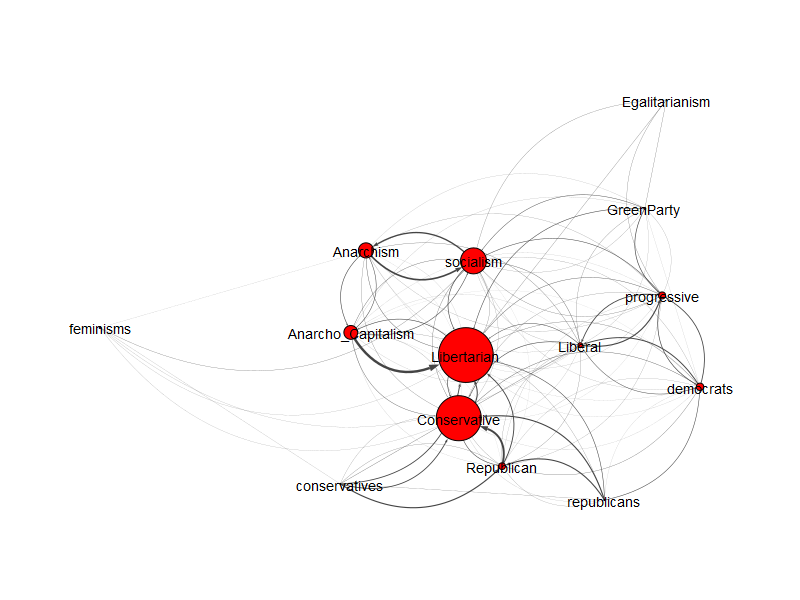
\includegraphics[width=\columnwidth]{img/ideology_network.png}
	\caption{\label{ideology_net} Different ideology-centric subreddits in our model}
\end{figure}

\section{Classification}

Now that we have acknowledged the presence of the echo chamber effect and how it can be more acute in polarized communities, we leverage this by attempting a classification of both the users and the communities based on the things they write. For simplicity, we are going to attempt to classify each text in the corpus of comments by it's left/right lean character.
As training data we sampled 25000 comments from each of r/democrats, r/Republican, r/Liberal and r/Conservative. Those are subs maintained by and for ideological stances.

\subsection{Natural Language Processing}

As a part of our analysis we performed sentiment analysis on all of the comments via nltk's sentiment package. For each comment we assign 4 metrics related to sentiment.

\begin{figure}[h]
	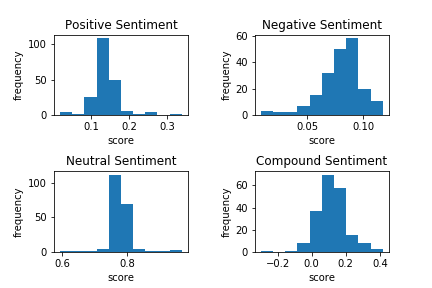
\includegraphics[width=\columnwidth,height=4cm]{img/sent_dist_total.png}
	\caption{Sentiment over our corpus}
\end{figure}

\subsection{Machine Learning}

In this approach we trained several stock ML models with engineered features from the body of the comments. Namely character count, word count, word density, uppercase word count, noun count, verb count, adjective count, adverb count, pronoun count, karma and sentiment. Fig. \ref{features} shows the different distributions of some of those values in the training data. Karma is pretty skewed towards left-leaning subs because those are bigger in size.

\begin{figure}[h]
	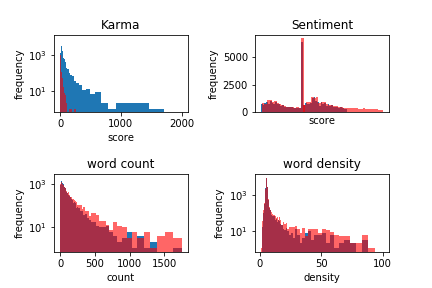
\includegraphics[width=\columnwidth]{img/training_stats.png}
	\caption{\label{features}Sentiment over training data}
\end{figure}

Here's the accuracy of our models in the test set (training data split 80-20) can be seen in fig. \ref{performance}.

\begin{figure}[h]
	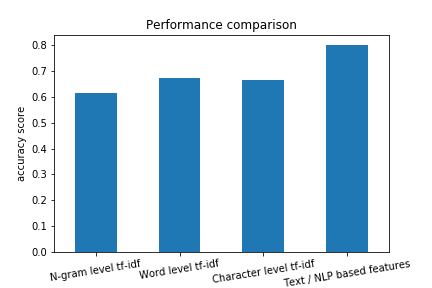
\includegraphics[width=\columnwidth]{img/performance.png}
	\caption{\label{performance} Performance of ML methods}
\end{figure}

Despite the high accuracy of some classifiers in the test set, in practice the classification wasn't very consistent. This might have to do with not ussing the actual content of the corpus but rather it's "gait" as it were.

We could have improved this by using the full content of the comments (word2vec) in training. Neural networks and great preprocessing (language filters, removing noise, etc) would be necessary for this approach though since this corpus is highly polluted "raw" text and not a curated one (like a novel, or newspapers).

\subsection{Topic Detection}

Our last approach was based on the fact that if the different parties maintain echo chambers, they would be talking mainly about different topics, curated by the moderators. Using spaCy we retrained the topic detection algorithm that we saw in the lectures with our two corpus (conservatives, liberals).

Unsurprisingly, this approach failed when setting the number of topics to 2. Both communities talk about seemingly the same, only that from different perspectives.

We believe though that this could be improved. Instead of trying to capture the main conversation topic in each group we could try to detect several of them, measure the topic distribution on each class and perform hypothesis testing on the topic distribution that a user/community shows to assign them a class. Unfortunately we ran out of time and didn't perform this set of experiments.

\section{Conclusion}

The immediate takeaway from this experiments is that, while the fact that echo chambers play a non-insignificant role in social dynamics nowadays might or might not be true, it is very likely that most individuals are exposed to a much more diverse set of political views and information sources now than they were in the pre-internet era. It is certainly possible to measure how much of an echo chamber an online community is thanks to big data, since we can see the symptoms, but it is a very complex problem that entails fine-tuning of algorithms for each kind of structure of mass social media.

We believe that this is really important since big challenges lie ahead of our generation: climate change, the rise of populism or the increasing inequality, both between nations and within borders, just to give a few examples. Fake news and crafted narratives have been a hot topic for a while, and while the internet has given certain agents the ability to reach a lot of people with minimal effort it has also provided huge advancements just for the fact that sharing information and knowledge is easier than ever in history. Understanding the way in which we communicate through that vast network is still key in order to come up with ways to protect ourselves from bad actors that might try to influence our reasoning.

\begin{figure*}[h]
	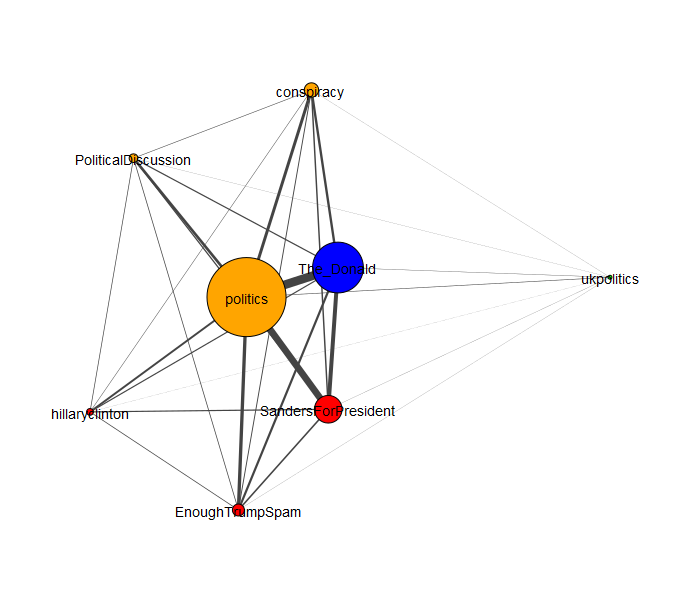
\includegraphics[width=\textwidth]{img/base_network.png}
	\caption{\label{base_net_big} Base network model}
\end{figure*}

\begin{figure*}[h]
	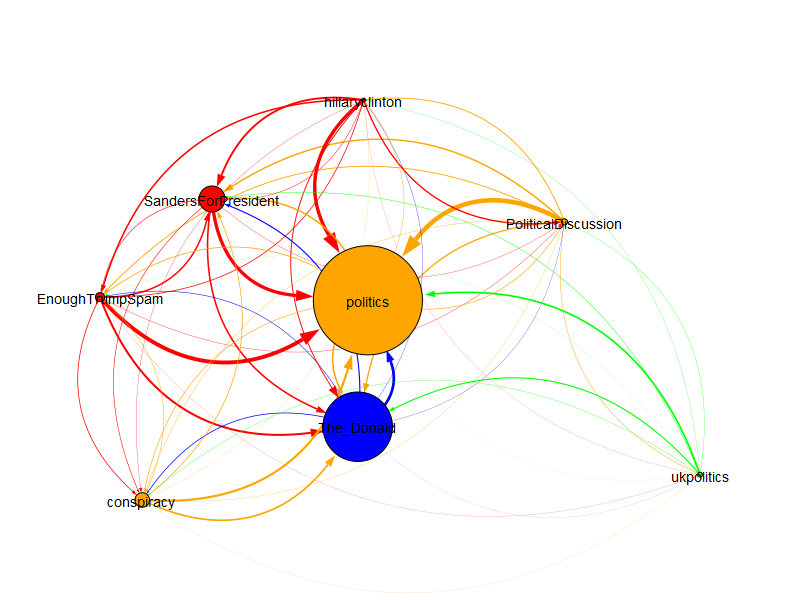
\includegraphics[width=\textwidth]{img/karma_model.png}
	\caption{\label{karma_net_big} Karma model in political subs}
\end{figure*}

\begin{figure*}[h]
	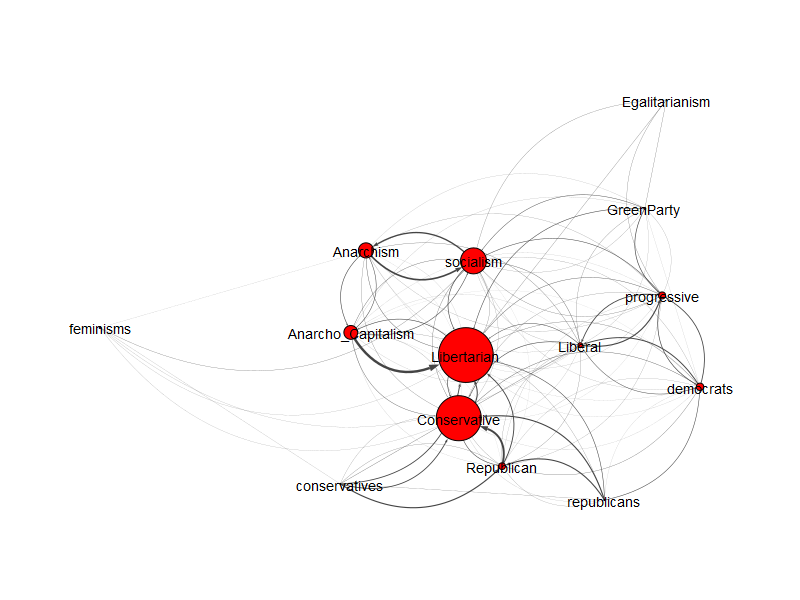
\includegraphics[width=\textwidth]{img/ideology_network.png}
	\caption{\label{ideology_net_big} Different ideology-centric subreddits in our model}
\end{figure*}


\end{document}
